\chapter{Working title}
\label{sec:something}


In the introduction to this project, we briefly discussed the scope and focus of the thesis. In figure/table .. we have displayed the complete list of structures, compositions and permutations of high-entropy silicides trialed throughout the duration of the project. \textbf{Make figure.} Amidst the large number of structures, we found particularly promising attributes of $(CrFeMnNi)Si_2$ (CFMN) SQSs based on the orthorombic crystal structure of $FeSi_2$, thus we will begin this section by presenting the results regarding this structure.

In this structure, each supercell consist of 48 total atoms, 32 of which is silicon, and the remaining 16 positions is equally distributed between Chromium, iron, manganese, and Nickel. The 5 distinct SQS supercells can be seen in figure (method/SQS). In table \ref{tab:FeSi2/CrFeMnNi_equal} we present a summary of the most relevant functional properties of the SQSs.

\begin{table}[]
\centering
\begin{tabular}{@{}cccc@{}}
\toprule
Structure  & Total energy/atom (eV) & Final magnetic moment (?) & Band gap (eV) \\ \midrule
\textbf{A} & −6,6080                & 4.0006                    & 0.0280        \\
\textbf{B} & −6,6138                & 3.9999                    & 0.0523        \\
\textbf{C} & −6,6063                & 4.0008                    & 0.0344        \\
\textbf{D} & −6,6155                & 4.0001                    & 0             \\
\textbf{E} & −6,6089                & 4.0000                    & 0.0495        \\ \bottomrule
\end{tabular}
\caption{Total energy per atom, final magnetic moment, and band gap (GGA) of 5 $Cr_4Fe_4Mn_4Ni_4Si_{32}$ SQSs based on $FeSi_2$}
\label{table:fesi2_summary}
\end{table}  

Bellow we have plotted the total density of states corresponding to the five distinct SQSs.

\begin{figure}
%\centering
\begin{subfigure}{0.5\textwidth}
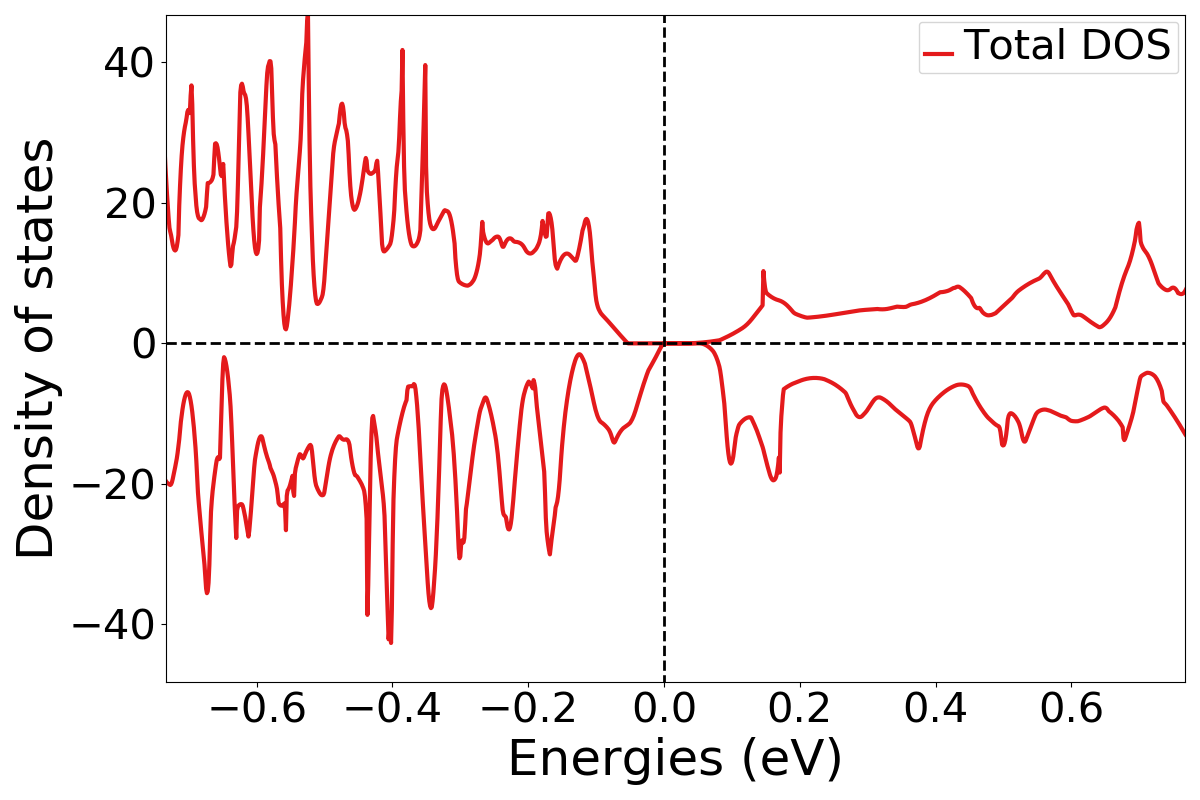
\includegraphics[width=\textwidth]{results/fesi2/DOS_A_toten.png}
\end{subfigure}
\begin{subfigure}{0.5\textwidth}
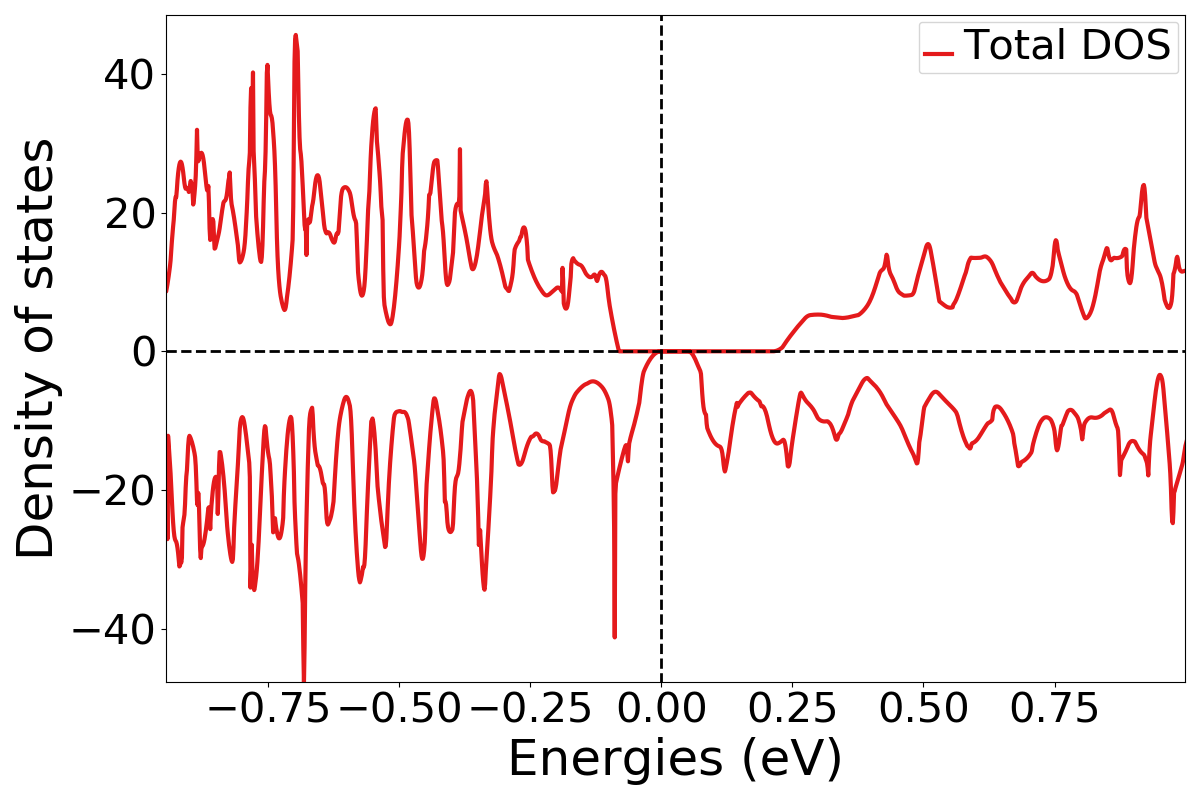
\includegraphics[width=\textwidth]{results/fesi2/DOS_B_toten.png}
\end{subfigure}
\begin{subfigure}{0.5\textwidth}
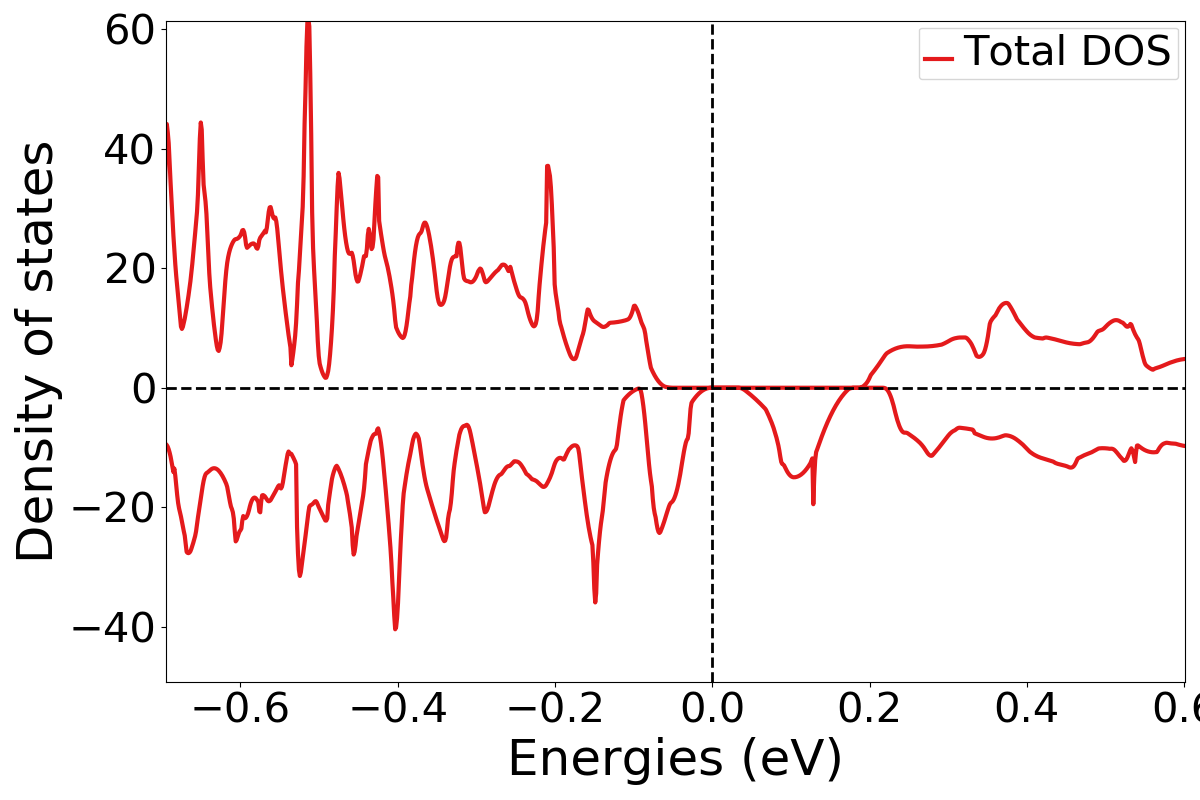
\includegraphics[width=\textwidth]{results/fesi2/DOS_C_toten.png}
\end{subfigure}
\begin{subfigure}{0.5\textwidth}
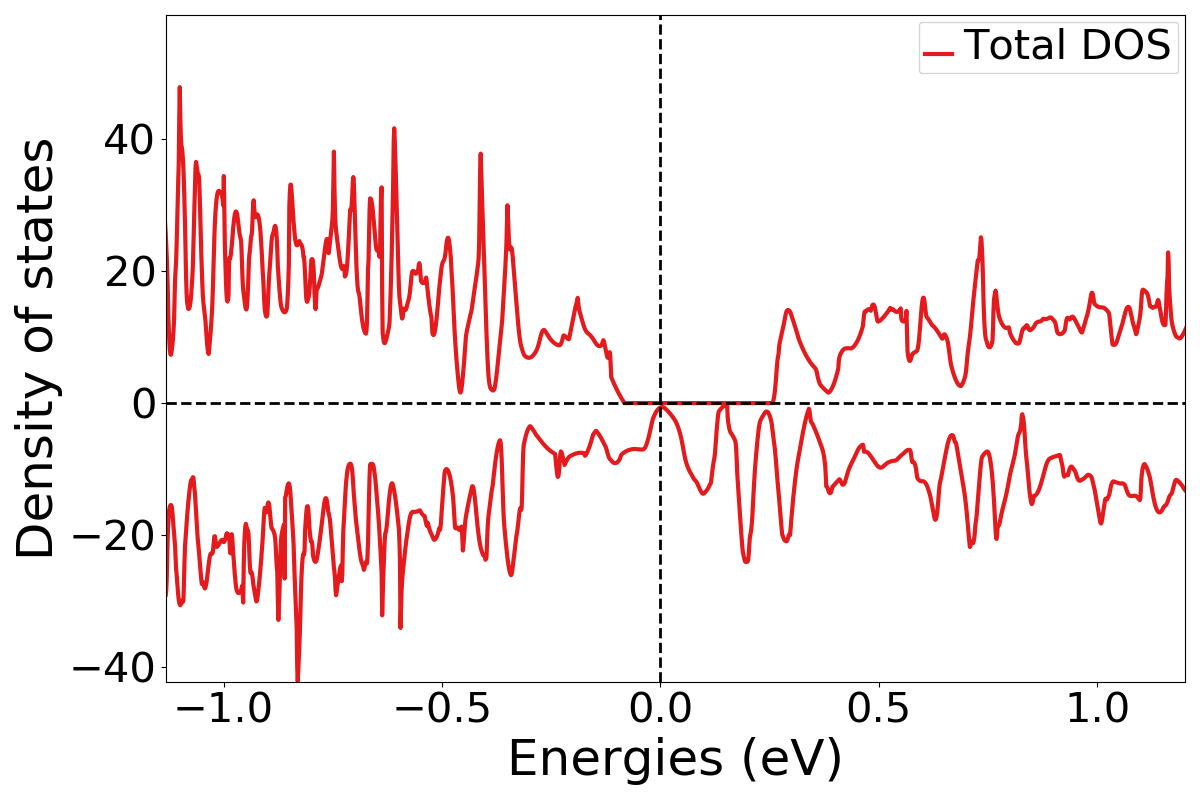
\includegraphics[width=\textwidth]{results/fesi2/DOS_D_toten.png}
\end{subfigure}
\begin{subfigure}{0.5\textwidth}
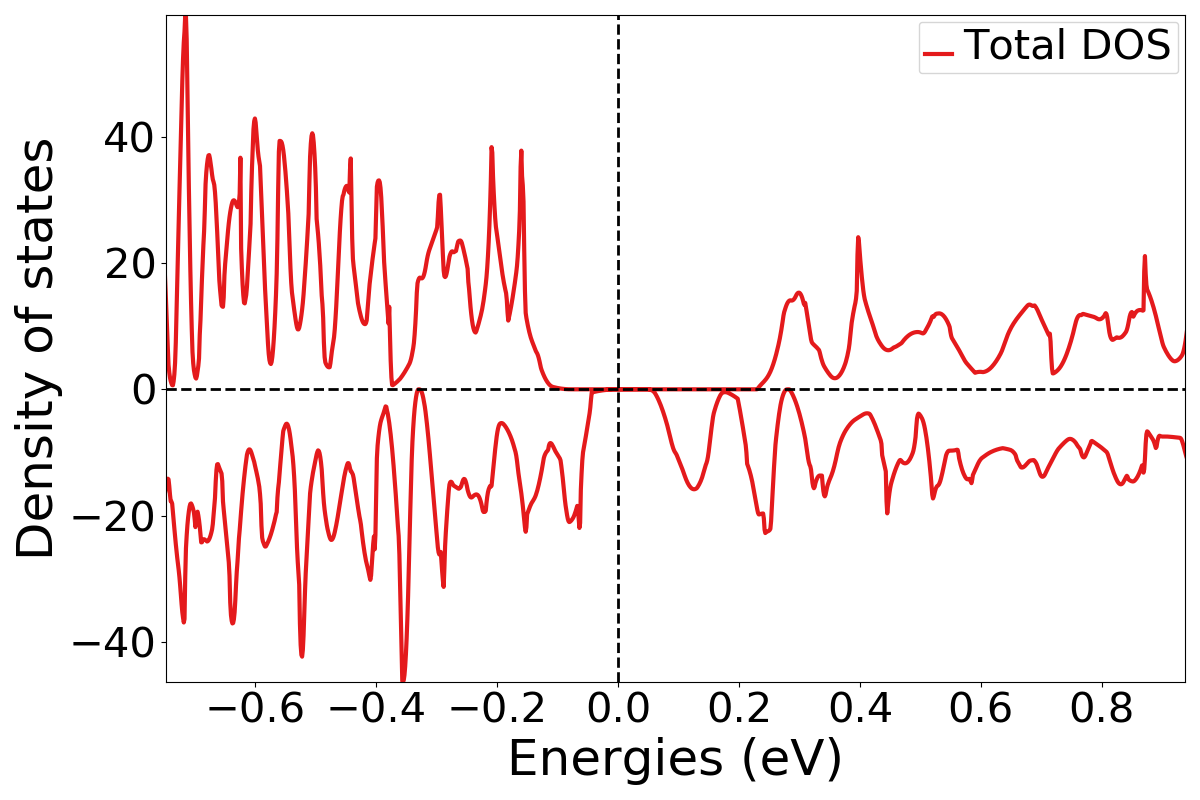
\includegraphics[width=\textwidth]{results/fesi2/DOS_E_toten.png}
\end{subfigure}
\caption{Density of states for structure A, B, C, D, E of $CFMNSi_2 (FeSi_2)$ SQSs (PBE GGA)}
\label{dos_fesi2_gga}
\end{figure}

\begin{table}[]
\centering
\begin{tabular}{@{}cccc@{}}
\toprule
Structure  & Spin-up & Spin-down & Total  \\ \midrule
\textbf{A} & 0.0814  & 0.0522    & 0.0281 \\
\textbf{B} & 0.2932  & 0.0523    & 0.0523 \\
\textbf{C} & 0.2355  & 0.0343    & 0.0343 \\
\textbf{D} & 0.3386  & 0         & 0      \\
\textbf{E} & 0.3078  & 0.0495    & 0.0495 \\ \bottomrule
\end{tabular}
\caption{Band gap (GGA) in spin up and spin down channels of CFMNSi2 structures}
\end{table}

\begin{table}[]
\centering
\begin{tabular}{@{}cccc@{}}
\toprule
Structure  & PBE    & SCAN   & HSE06  \\ \midrule
\textbf{A} & 0.0281 & 0.0000 & 0.1493 \\
\textbf{B} & 0.0523 & 0.0890 & 0.1506 \\
\textbf{C} & 0.0344 & 0.0690 & 0.0649 \\
\textbf{D} & 0.0000 & 0.0000 & 0.0000 \\
\textbf{E} & 0.0495 & 0.1048 & 0.1439 \\ \bottomrule
\end{tabular}
\caption{Band gap of $CFMN (FeSi_2)$ SQSs with GGA (PBE), meta-GGA (SCAN) and hybrid-functionals (HSE06). \textbf{Add footnote to explain the uncertainty in these results regarding smearing type and width, and DOS and EIGENVAL}}
\end{table}
